\documentclass{beamer}
\usepackage[latin1]{inputenc}
\usetheme{Warsaw}
\title[Dynamically kicking balls]{Dynamically kicking balls with a
Nao}
\author{Inge Becht\\ Maarten de Jonge\\ Richard Pronk}
\institute{University of Amsterdam}
\date{June 24, 2012}
\begin{document}

\begin{frame}
\titlepage
\end{frame}

\begin{frame}{Goal of The Project}
    \begin{itemize}
        \item{Making a nao able to kick a ball dynamically}
        \item{Nao plans a kick by making a tradeoff between
             accuracy and stableness}
        \item{Integrating solution  into current Dutch Nao Team code}
    \end{itemize}
\end{frame}

\begin{frame}{What is a Nao?}
    \begin{itemize}
        \item{Humanoid robot}
        \item{Used in the Standard Platform League}
    \end{itemize}
     \begin{figure}[H] 
        \begin{center}
            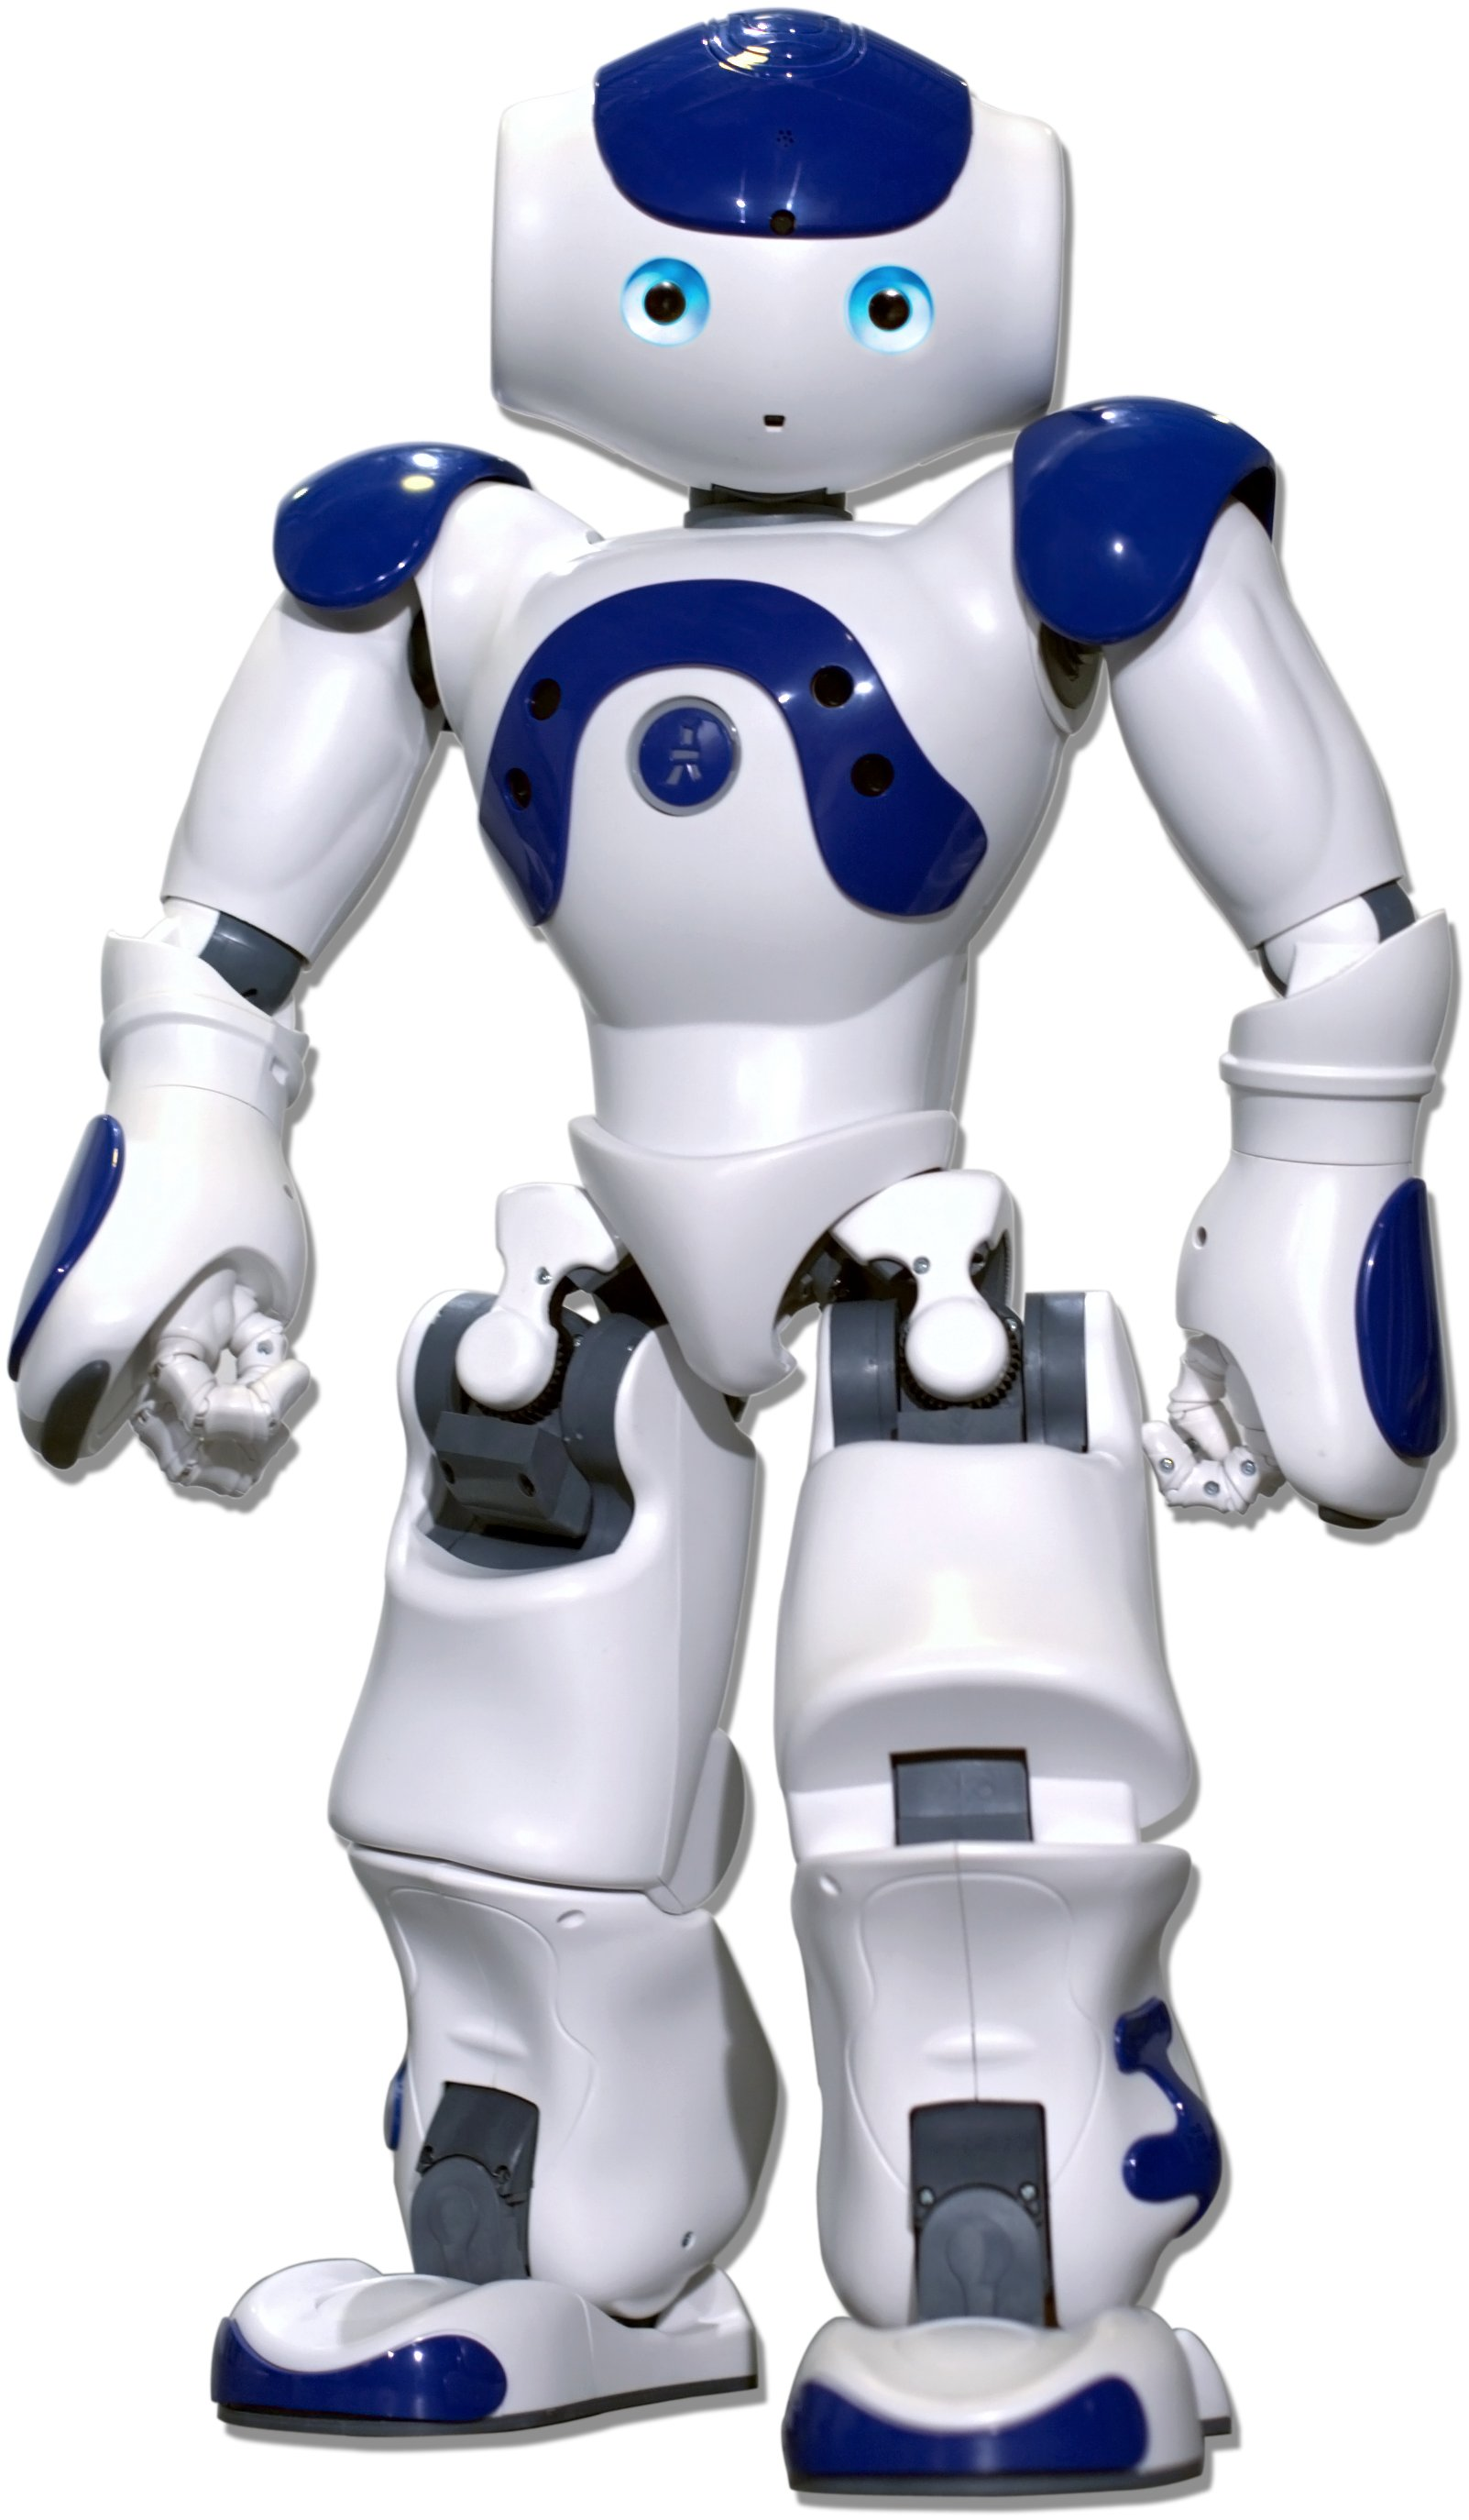
\includegraphics[scale=0.2]{nao.jpg}
            \caption{Nao}
        \end{center}
    \end{figure}  
\end{frame}

\begin{frame}{Why?}
    \begin{itemize}
        \item{Covers same difficulties as walking, but simpler}
        \item{Keyframe motion is brittle}
        \item{More robust to environmental factors}
            \begin{itemize}
                \item{Interference by other Naos}
                \item{Compensation for hot joints}
            \end{itemize}
        \item{Will Help the Dutch Nao Team in their next competition}
    \end{itemize}
\end{frame}

\begin{frame}{Possible?}
    \begin{itemize}
        \item{Yes, But quite a lot of work}
        \item{}
    \end{itemize}
\end{frame}

\begin{frame}{Data gathered}
    \begin{itemize}
        \item{Team papers about dynamical movement in a Nao} 
        \item{None containing the exact problem we need to tackle}
    \end{itemize}
\end{frame}

\begin{frame}{All tasks}
    \begin{itemize}
        \item{Calculating Center of Mass (Currently working on)}
        \item{Calculating the Suport polygon}
        \item{Achieving a inverse kinematica space}
        \item{Evaluating possible kicking motions to be stable enough before
            execution}
    \end{itemize}
\end{frame}

\begin{frame}{Current planning}
    \begin{itemize}
    \item{This week: Calculating Center of Mass on a Nao}
    \item{Two week break: traveling to Mexico}
    \item{Second week: looking at solving the inverse kinematics chain}
    \item{Third week: Finding out which kicks can be applied and which not }
    \item{Forth week: finishing up all parts and calculating the code} 
    \end{itemize}
\end{frame}

\end{document}
